\chapter{Desarrollo e implementación}

Una vez elegidas todas las herramientas y tecnologías necesarias para el desarrollo del sistema, se procede a la fase de implementación. En esta sección se detallan los componentes del backend, así como el uso de contenedores Docker para la base de datos y su administración.

\section{Desarrollo del backend}

\subsection{Docker}

Para facilitar la gestión y despliegue de la base de datos se ha configurado \textbf{PostgreSQL} en un contenedor Docker, acompañado de \textbf{pgAdmin} como herramienta de administración de base de datos. Esta estructura en contenedores asegura que el entorno sea replicable y consistente en distintas fases del desarrollo y despliegue.

La configuración de estos servicios en Docker se define en un archivo `docker-compose.yml`, que permite instanciar tanto la base de datos como la interfaz de administración en contenedores separados pero conectados entre sí. A continuación, se presenta el contenido del archivo `docker-compose.yml` utilizado para la configuración:


\begin{lstlisting}[caption={Archivo docker-compose.yml para PostgreSQL y pgAdmin}, label={lst:docker-compose}]
	version: '3.8'
	
	services:
	db:
	image: postgres
	restart: always
	shm_size: 128mb
	environment:
	POSTGRES_USER: root
	POSTGRES_PASSWORD: root
	POSTGRES_DB: postgres
	ports:
	- "5432:5432"
	volumes:
	- postgres_data:/var/lib/postgresql/data
	
	pgadmin:
	image: dpage/pgadmin4
	restart: always
	environment:
	PGADMIN_DEFAULT_EMAIL=admin@admin.com
	PGADMIN_DEFAULT_PASSWORD=root
	ports:
	- "5050:80"
	volumes:
	- pgadmin_data:/var/lib/pgadmin
	
	volumes:
	postgres_data: 
	driver: local
	pgadmin_data: 
	driver: local
\end{lstlisting}


El servicio db se encarga de ejecutar la instancia de PostgreSQL configurada para estar accesible en el puerto 5432 de la máquina local. Además, utiliza un volumen persistente \texttt{postgres} data para asegurar que los datos de la base de datos se mantengan incluso si el contenedor se detiene o reinicia.

Por otro lado, el servicio pgadmin proporciona una interfaz gráfica para la administración de la base de datos, accesible en el puerto 5050 de la máquina local. Este servicio también utiliza un volumen persistente \texttt{pgadmin} data para almacenar sus configuraciones de forma persistente. \\

Esta configuración en Docker permite separar los entornos de desarrollo y producción, facilitando la administración y el despliegue seguro de la base de datos y sus herramientas de administración.

\subsection{Prisma}
Para llevar a cabo la conexión entre Prisma y el contenedor de Docker donde está desplegada la base de datos PostgreSQL, se ha creado el archivo schema.prisma. Este archivo define el modelo de datos utilizado en el sistema y permite a Prisma interactuar con la base de datos de manera estructurada y eficiente.

Después de configurar el esquema en schema.prisma, se procedió a instalar el paquete \url{@prisma/client}. Este cliente permite realizar consultas a la base de datos de forma sencilla y directa desde el código de Node.js, utilizando Prisma como ORM. La instalación y configuración del cliente Prisma permitieron verificar que la conexión con PostgreSQL y con pgAdmin estaba funcionando correctamente, lo que permitió visualizar y administrar los datos almacenados tanto en pgAdmin como en Prisma.

La verificación de esta conexión incluyó la comprobación de que los datos ingresados o modificados en la base de datos a través de Prisma aparecían correctamente en pgAdmin y viceversa, confirmando así la correcta sincronización y funcionalidad de ambos entornos. Como resultado de esta configuración y de la estructura de schema.prisma, se obtuvo la estructura de tablas que se muestra en la imagen, donde se representa el modelo de datos en sus diferentes entidades y relaciones, necesarias para cumplir con los requisitos del sistema.
\newpage

\begin{figure}[h!]
	\centering
	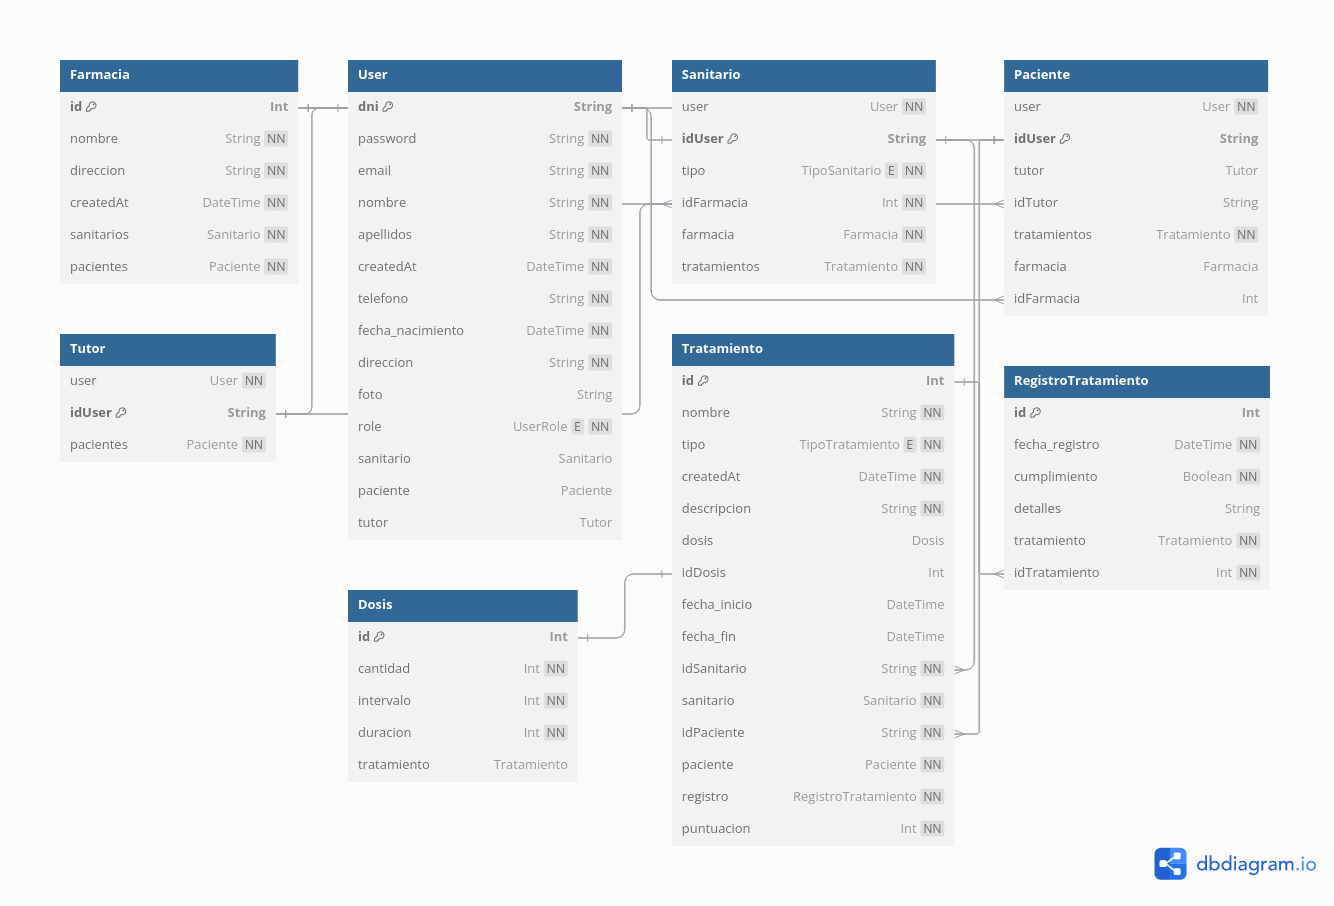
\includegraphics[width=1\textwidth]{imagenes/tablasbd.png}
	\caption{Tablas de la base de datos.}
\end{figure}

El modelo de datos establece varias relaciones clave: una farmacia puede tener múltiples sanitarios y pacientes asociados, lo que organiza a ambos grupos bajo un establecimiento específico. Cada sanitario y paciente está registrado como usuario en el sistema, permitiendo gestionar distintos roles y accesos. Los tutores pueden estar vinculados a pacientes que requieren asistencia, facilitando el seguimiento. Además, un sanitario es responsable de los tratamientos de los pacientes, cada uno de los cuales tiene su pauta de dosis y registros de adherencia, lo que permite monitorizar la evolución del tratamiento.

\subsection{Fastify, desarrollo de API}

Para configurar Fastify en este proyecto se han establecido cinco componentes principales: controladores, plugins, rutas, tests y utils. A continuación, se explica brevemente la función de cada uno y se muestra un ejemplo de código asociado.

\begin{itemize}
	\item \textbf{Controladores}. Los controladores gestionan la lógica de negocio de las operaciones solicitadas por el cliente. En este caso, el controlador maneja la creación de usuarios, validando roles y permisos de acceso según el tipo de usuario que solicita la acción.

\begin{lstlisting}[caption={Ejemplo de controlador para crear un usuario}, label={lst:createUser}]
	const createUser = async (req, reply) => {
		try {
			const { dni, email, password, nombre, apellidos, fechaNac, telefono, direccion, role, tipoSanitario, idFarmacia, foto, dniPaciente } = req.body
			const userCreator = req.user
			
			const existingUser = await prisma.user.findUnique({
				where: { dni }
			})
			
			const fechaNacimiento = new Date(fechaNac)
			if (isNaN(fechaNacimiento.getTime())) {
				return reply.status(400).send({ error: 'Fecha de nacimiento no es válida.' })
			}
			
			if (existingUser) return reply.status(400).send({ error: 'Ya existe un usuario con este DNI.' })
			
			let allowedRoles = []
			
			if (userCreator.role === ROLES.ADMIN) {
				allowedRoles = createUserPermissions[ROLES.ADMIN]
			} else if (userCreator.role === ROLES.SANITARIO) {
				if (!userCreator.sanitario) {
					userCreator.sanitario = await prisma.sanitario.findUnique({
						where: { idUser: userCreator.dni }
					})
					
					if (!userCreator.sanitario) 
					return reply.status(400).send({ error: 'El usuario sanitario no tiene información de tipo de sanitario.' })
					
				}
				allowedRoles = createUserPermissions[userCreator.sanitario.tipo] || []
				
			} else {
				return reply.status(403).send({ error: 'UNAUTHORIZED. Only an ADMIN or SANITARIO can create users.' })
			}
			
			if (!allowedRoles.includes(role)) {
				return reply.status(403).send({ error: 'UNAUTHORIZED. You are not allowed to create a user with this role.' })
			}
			
			if (role === ROLES.SANITARIO && !tipoSanitario) {
				return reply.status(400).send({ error: 'El tipo de sanitario es requerido.' })
			}
			
			if (role === ROLES.SANITARIO && !Object.values(TIPO_SANITARIO).includes(tipoSanitario)) {
				return reply.status(400).send({ error: 'El tipo de sanitario no es válido.' })
			}
			
			if (role === ROLES.SANITARIO && !idFarmacia) {
				return reply.status(400).send({ error: 'El id de la farmacia es requerido para sanitarios.' })
			}
			
			if (idFarmacia) {
				const farmacia = await prisma.farmacia.findUnique({
					where: { id: idFarmacia }
				}) 
				if (!farmacia) return reply.status(400).send({ error: 'La farmacia no existe.' })
			}
			
			if (role === ROLES.TUTOR) {
				if (!dniPaciente) {
					return reply.status(400).send({ error: 'El DNI del paciente es requerido.' })
				}
				
				const existingPatient = await prisma.paciente.findUnique({
					where: { idUser: dniPaciente }
				})
				if (!existingPatient) return reply.status(400).send({ error: 'El paciente no existe.' })
			}
			
			const hashedPassword = await hashPassword(password)
			
			const newUser = await prisma.user.create({
				data: {
					dni,
					email,
					password: hashedPassword,
					nombre,
					apellidos,
					fecha_nacimiento: fechaNacimiento,
					telefono,
					direccion,
					foto,
					role,
					sanitario: role === ROLES.SANITARIO ? {
						create: {
							tipo: tipoSanitario,
							idFarmacia
						}
					} : undefined,
					tutor: role === ROLES.TUTOR ? {
						create: {
							pacientes: { connect: { idUser: dniPaciente } } 
						}
					} : undefined,
					paciente: role === ROLES.PACIENTE ? {
						create: {
							idFarmacia
						}
					} : undefined
				}
			})
			
			if (role === ROLES.TUTOR) {
				await prisma.paciente.update({
					where: { idUser: dniPaciente }, 
					data: { idTutor: newUser.dni } 
				})
			}
			
			return reply.status(201).send({ message: 'User created successfully.', user: newUser })
			
		} catch (error) {
			console.error(error)
			reply.status(500).send({ error: 'Error creating user.' })
		}
	}
\end{lstlisting}

\newpage

\item \textbf{Plugins o \textit{Middleware}}. Los plugins extienden la funcionalidad de Fastify. En este ejemplo, se ha configurado un plugin para manejar JWT (JSON Web Tokens) y así asegurar rutas.

\begin{lstlisting}[caption={Plugin para JWT}, label={lst:pluginJWT}]
	import fp from 'fastify-plugin'
	import jwt from '@fastify/jwt'
	
	export default fp(async function (fastify, options) {
		fastify.register(jwt, {
			secret: process.env.JWT_SIGNING_SECRET
		})
		
		fastify.decorate("jwtAuth", async function (request, reply) {
			try {
				await request.jwtVerify()
			} catch (err) {
				reply.status(401).send({ err })
			}
		})
		
	})
\end{lstlisting}

\item \textbf{Rutas}. Las rutas definen los puntos de acceso a los controladores. Se utiliza preValidation con jwtAuth para proteger las rutas, asegurando que solo usuarios autenticados puedan acceder.

\begin{lstlisting}[caption={Definición de rutas para usuarios}, label={lst:userRoutes}]
	import userController from '../controllers/userController.js'
	
	async function userRouters(fastify, options) {
		fastify.post('/users/create', { preValidation: [fastify.jwtAuth] }, userController.createUser)               
		fastify.get('/users/:dni', { preValidation: [fastify.jwtAuth] }, userController.getUserByDNI)         
		fastify.get('/users', { preValidation: [fastify.jwtAuth] }, userController.getAllUsers)               
		fastify.put('/users/:dni', { preValidation: [fastify.jwtAuth] }, userController.updateUser)          
		fastify.delete('/users/:dni', { preValidation: [fastify.jwtAuth] }, userController.deleteUser)        
		fastify.get('/users/sanitarios/:dni', { preValidation: [fastify.jwtAuth] }, userController.getSanitarioData) 
		fastify.get('/users/pacientes/:dni', { preValidation: [fastify.jwtAuth] }, userController.getPacienteData)   
		fastify.get('/users/tutores/:dni', { preValidation: [fastify.jwtAuth] }, userController.getTutorData)  
		fastify.get('/users/pacientes/sinfarmacia', { preValidation: [fastify.jwtAuth] }, userController.getPacientesSinFarmacia)
		fastify.put('/users/:dni/password', { preValidation: [fastify.jwtAuth] }, userController.updatePassword)
	}
	
	export default userRouters
\end{lstlisting}
\newpage

\item \textbf{Tests}. Los tests validan la funcionalidad del sistema, asegurando que las operaciones cumplen con las expectativas. En este ejemplo, se verifica que un farmacéutico pueda crear un tratamiento farmacológico para un paciente.

\begin{lstlisting}[caption={Ejemplo de test para creación de tratamiento}, label={lst:createTreatmentTest}]
	it('Debería permitir al farmacéutico crear un tratamiento farmacológico para un paciente', async () => {
		const farmaceuticoLogin = await fastify.inject({
			method: 'POST',
			url: '/api/login',
			payload: { dni: '33445566G', password: 'farmaceutico567' }
		})
		expect(farmaceuticoLogin.statusCode).to.equal(200)
		const farmaceuticoToken = JSON.parse(farmaceuticoLogin.payload).token
		
		const tratamientoFarmacologicoResponse = await fastify.inject({
			method: 'POST',
			url: '/api/tratamientos/create',
			headers: { Authorization: `Bearer ${farmaceuticoToken}` },
			payload: {
				nombre: 'Tratamiento Antibiotico',
				tipo: 'FARMACOLOGICO',
				descripcion: 'Tratamiento para infección',
				idPaciente: pacienteId1,
				dosis: {
					cantidad: 500,
					intervalo: 8,
					duracion: 10
				}
			}
		})
		expect(tratamientoFarmacologicoResponse.statusCode).to.equal(201)
		const tratamiento = JSON.parse(tratamientoFarmacologicoResponse.payload)
		tratamientoId1 = tratamiento.id
	})
\end{lstlisting}


\item \textbf{Utils}. Los utils agrupan funciones de utilidad que se utilizan en distintos puntos del código. En este caso, se incluyen funciones para encriptar y comparar contraseñas.
\begin{lstlisting}[caption={Funciones de utilidad para contraseñas}, label={lst:utilsPassword}]
	import bcrypt from 'bcrypt';
	
	const SALT_ROUNDS = 12
	
	export async function hashPassword(password) {
		try {
			return await bcrypt.hash(password, SALT_ROUNDS)
		} catch (error) {
			console.error('Error hashing password:', error)
			throw new Error('Failed to hash password')
		}
	}
	
	export const comparePassword = async (password, hashedPassword) => {
		return bcrypt.compare(password, hashedPassword)
	}
\end{lstlisting}


\item \textbf{Configuración del servidor}. En el archivo \texttt{server.js} se configura el servidor Fastify, que actúa como el núcleo de la aplicación, integrando diferentes funcionalidades a través de plugins, rutas y configuraciones específicas. \\

En \texttt{server.js} primero se importa y configura Fastify, iniciando el servidor con un logger detallado para rastrear eventos y errores. Luego, se registra el plugin cors, permitiendo el acceso desde distintas fuentes con los métodos HTTP especificados. También se habilita el plugin JWT para manejar la autenticación con tokens, asegurando que solo los usuarios autorizados puedan acceder a ciertas rutas.

A continuación, se registra un parser para solicitudes en formato JSON. Después se configuran las rutas principales del servidor (farmaciaRoutes, userRoutes, tratamientoRoutes y authRoutes), todas accesibles bajo el prefijo /api. Finalmente, se define una ruta por defecto para probar el funcionamiento del servidor y se implementa una función para iniciar el servidor en el puerto indicado, gestionando cualquier error que ocurra al iniciar.

\begin{lstlisting}[caption={Archivo server.js - Configuración del servidor Fastify}, label={lst:server-js}]
	import Fastify from 'fastify'
	import { PORT } from './config/init.js'
	import cors from '@fastify/cors'; 
	import farmaciaRoutes from './routes/farmaciaRoutes.js'
	import userRoutes from './routes/userRoutes.js'
	import tratamientoRoutes from './routes/tratamientoRoutes.js'
	import authRoutes from './routes/authRoutes.js'
	import jwtPlugin from './plugins/jwtPlugin.js'
	
	const fastify = Fastify({
		logger: {
			level: 'trace',
			transport: {
				target: 'pino-pretty',
			}
		}
	})
	

	fastify.register(cors, { 
		origin: true, 
		methods: ['POST', 'GET', 'PUT', 'DELETE', 'OPTIONS'],
	})
	
	fastify.register(jwtPlugin)
	
	// Parser para contenido JSON
	fastify.addContentTypeParser('application/json', { parseAs: 'string' }, fastify.getDefaultJsonParser('strict'))
	
	fastify.register(farmaciaRoutes, { prefix: '/api' })
	fastify.register(userRoutes, { prefix: '/api' })
	fastify.register(tratamientoRoutes, { prefix: '/api' })
	fastify.register(authRoutes, { prefix: '/api' })
	
	// Ruta por defecto
	fastify.get('/', async function handler (request, reply) {
		return { hello: 'world' }
	})
	
	const startServer = async () => {
		try {
			await fastify.listen({ port: PORT })
			console.log(`Server is running on port ${ PORT }`)
			
		} catch (err) {
			fastify.log.error(err)
			process.exit(1)
		}
	}
	
	export default fastify
	startServer()
\end{lstlisting}


\end{itemize}

\subsection{Dependencias de Node.js}
 Las dependencias son módulos externos que un proyecto necesita para funcionar correctamente. Estas se especifican en el archivo \texttt{package.json} bajo las secciones \texttt{dependencies} y \texttt{devDependencies}.
\begin{itemize} 
	\item \textbf{@fastify/cors}: Permite configurar CORS (Cross-Origin Resource Sharing) en Fastify, lo que habilita solicitudes desde distintos dominios y métodos HTTP específicos. 
	\item \textbf{@fastify/jwt}: Gestiona la autenticación mediante JSON Web Tokens (JWT), proporcionando seguridad al sistema al verificar usuarios. 
	\item \textbf{@prisma/client}: Cliente de Prisma para interactuar con la base de datos para realizar consultas y operaciones sobre el esquema definido en \texttt{schema.prisma}. 
	\item \textbf{bcrypt}: Utilizado para encriptar contraseñas.
	\item \textbf{fastify-plugin}: Facilita la creación y uso de plugins en Fastify. 
	\item \textbf{pino-pretty}: Formatea los logs generados por Fastify para hacerlos más legibles durante el desarrollo. 
	\item \textbf{chai}: Biblioteca de aserciones para escribir pruebas, proporcionando múltiples estilos de aserción para verificar resultados. 
	\item \textbf{mocha}: Marco de pruebas que permite ejecutar y estructurar pruebas, facilitando la verificación de la funcionalidad del sistema.  
	\item \textbf{prisma-dbml-generator}: Genera diagramas de entidad-relación (ERD) en formato DBML, visualizando el modelo de datos definido en Prisma.
\end{itemize}

\subsection{Flujo de peticiones a API} El flujo de una petición a la API en Fastify comienza cuando un cliente envía una solicitud a una ruta específica, como POST \texttt{/api/users/create}. Primero, la ruta definida en el archivo de rutas (por ejemplo, userRoutes.js) intercepta la solicitud. Si la ruta está protegida, se aplica una pre-validación, utilizando el plugin de autenticación JWT (como jwtPlugin.js), que verifica que el cliente esté autenticado. Una vez autenticado, el controlador correspondiente (en este caso, createUser en userController.js) se encarga de procesar la lógica principal de la solicitud, como validar datos y realizar operaciones en la base de datos usando Prisma. Finalmente, la respuesta se envía al cliente, indicando el éxito o el error de la operación. Este flujo asegura un manejo estructurado y seguro de las solicitudes en la API.

\newpage

\subsection{Organización de directorios} Finalmente, la estructura de directorios para el backend se muestra como sigue:
\begin{figure}[h!]
	\centering
	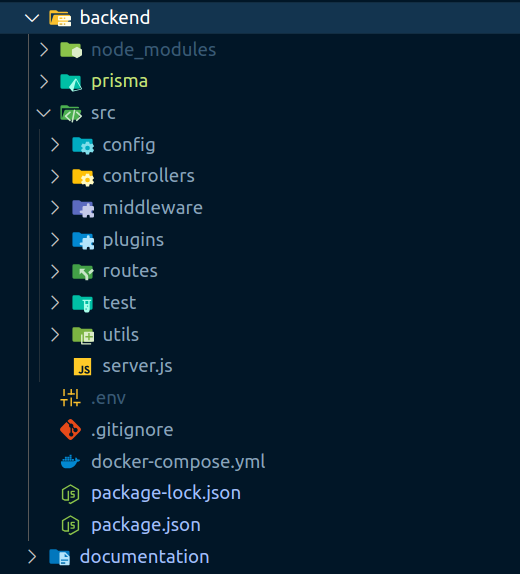
\includegraphics[width=0.5\textwidth]{imagenes/orgback.png}
	\caption{Directorios del backend.}
\end{figure}



\section{Desarrollo del frontend}

\subsection{Desarrollo del frontend con Astro}

En el desarrollo del frontend se ha utilizado Astro y se ha configurado para que tenga un layout base que permita establecer una estructura y diseño consistentes en todas las páginas de la aplicación. Este layout se configura en el archivo \texttt{Layout.astro} y contiene componentes comunes como la barra de navegación, pie de página y verificación de autenticación.

\subsubsection{Configuración del layout base}

El layout base incluye los componentes esenciales y define cuándo deben mostrarse, basándose en la ruta actual. A continuación se presenta el código del archivo \texttt{Layout.astro}:

\begin{lstlisting}[language=html, caption={Layout base en Astro}]
	---
	import Navbarreact from "../components/ui/Navbar";
	import Footer from "../components/ui/footer.astro";
	import AuthCheck from "../components/sections/checks/AuthCheck";
	
	interface Props {
		title: string;
	}
	
	const { title } = Astro.props;
	const currentPath = Astro.url.pathname;
	const showNavbar = currentPath !== "/" && currentPath !== "/login";
	const showLimit = showNavbar;
	const authCheck = showNavbar;
	---
	
	<!doctype html>
	<html lang="es" class="lenis lenis-smooth scroll-pt-5">
	<head>
	<meta charset="UTF-8" />
	<meta name="description" content="Astro description" />
	<meta name="viewport" content="width=device-width" />
	<link rel="icon" type="image/svg+xml" href="/favicon.svg" />
	<meta name="author" content="VIDICAN, MIHNEA IOAN" />
	<meta name="generator" content={Astro.generator} />
	<title>{title}</title>
	</head>
	<style>
	html {
		overflow-y: scroll;
	}
	</style>
	<body class="bg-base-100 w-full">
	<div class="grid min-h-screen grid-rows-[auto_1fr_auto]">
	{showNavbar && <Navbarreact client:load />}
	{authCheck && <AuthCheck client:load/>}
	
	<main>
	<div class={showLimit ? "max-w-screen-xl mx-auto" : ""}>
	<slot />
	</div>
	</main>
	
	<Footer />
	</div>
	</body>
	<script>
	import "../../assets/scripts/lenisSmoothScroll.js";
	</script>
	</html>
\end{lstlisting}

En este layout, se configuran los componentes comunes \texttt{Navbarreact}, \texttt{Footer}, y \texttt{AuthCheck}, que se muestran solo en determinadas rutas. La etiqueta \texttt{<slot />} permite incluir el contenido de cada vista específica dentro de esta estructura.

\subsubsection{Uso del layout en una vista específica}

Para cada página, se utiliza el layout importándolo y envolviendo el contenido dentro de él. A continuación, se muestra cómo se utiliza el layout en la página de inicio de sesión, \texttt{login.astro}:

\begin{lstlisting}[language=html, caption={Uso del Layout en login.astro}]
	---
	import Layout from "../layouts/Layout.astro";
	import LoginForm from "../components/sections/LoginForm.jsx";
	---
	
	<Layout title="Inicio de sesión">
	<LoginForm client:load />
	</Layout>
\end{lstlisting}

\begin{itemize}
	\item Aquí, el componente \texttt{LoginForm} se incluye dentro del layout, configurando así la página de inicio de sesión con el mismo estilo y estructura que el layout base.
	\item Esto permite mantener una estructura común en toda la aplicación.
\end{itemize}

\subsection{Uso de React}

Para añadir interactividad en el frontend, como se ha mencionado previamente, se ha utilizado \textbf{React}. A continuación se muestra un ejemplo del archivo \texttt{TratamientosForm.jsx}, un componente que permite a un sanitario, bien sea un farmacéutico o técnico de farmacia, crear un tratamiento específico para un paciente. Este formulario incluye validación de datos y mensajes de éxito o error según el resultado de la petición.

\begin{lstlisting}[caption={TratamientoForm.jsx - Formulario de creación de tratamiento para un paciente}]
	import { useState, useEffect } from "react";
	import SanitarioCheck from "../checks/SanitarioCheck";
	
	const TratamientoForm = () => {
		const [nombre, setNombre] = useState("");
		const [descripcion, setDescripcion] = useState("");
		const [tipo, setTipo] = useState("");
		const [dosis, setDosis] = useState({ cantidad: "", intervalo: "", duracion: "" });
		const [fechaFin, setFechaFin] = useState("");
		const [idFarmacia, setIdFarmacia] = useState(null);
		const [pacientes, setPacientes] = useState([]);
		const [idPaciente, setIdPaciente] = useState("");
		const [isLoading, setIsLoading] = useState(false);
		const [errorMessage, setErrorMessage] = useState("");
		const [successMessage, setSuccessMessage] = useState("");
		
		useEffect(() => {
			const fetchSanitarioData = async () => {
				const user = JSON.parse(sessionStorage.getItem("user"));
				if (user && user.dni) {
					try {
						const token = sessionStorage.getItem("jwtToken");
						const response = await fetch(`http://localhost:3000/api/users/sanitarios/${user.dni}`, {
							headers: { Authorization: `Bearer ${token}` },
						});
						const data = await response.json();
						if (response.ok) {
							setIdFarmacia(data.idFarmacia);
							fetchPacientes(data.idFarmacia, token);
						} else {
							setErrorMessage(data.error || "No se pudo obtener el ID de la farmacia.");
						}
					} catch (error) {
						console.error("Error al obtener los datos del sanitario:", error);
						setErrorMessage("Error de conexión al obtener los datos del sanitario.");
					}
				} else {
					setErrorMessage("No se pudo obtener el DNI del usuario logeado.");
				}
			};
			
			fetchSanitarioData();
		}, []);
		
		const fetchPacientes = async (farmaciaId, token) => {
			try {
				const response = await fetch(`http://localhost:3000/api/farmacias/${farmaciaId}/pacientes`, {
					method: "GET",
					headers: { Authorization: `Bearer ${token}` },
				});
				const data = await response.json();
				if (response.ok) {
					setPacientes(data);
				} else {
					setErrorMessage(data.error || "Error al obtener los pacientes.");
				}
			} catch (error) {
				console.error("Error fetching pacientes:", error);
				setErrorMessage("Hubo un problema con la conexión. Inténtelo de nuevo más tarde.");
			}
		};
		
		const validateForm = () => {
			if (!nombre || !descripcion || !tipo || !idPaciente) {
				setErrorMessage("Todos los campos son obligatorios.");
				return false;
			}
			if (tipo === "FARMACOLOGICO" && (!dosis.cantidad || !dosis.intervalo || !dosis.duracion)) {
				setErrorMessage("Todos los campos de dosis son obligatorios para un tratamiento farmacológico.");
				return false;
			}
			if (tipo === "NO_FARMACOLOGICO" && !fechaFin) {
				setErrorMessage("La fecha de fin es obligatoria para un tratamiento no farmacológico.");
				return false;
			}
			setErrorMessage("");
			return true;
		};
		
		const handleSubmit = async (e) => {
			e.preventDefault();
			if (!validateForm()) return;
			
			setIsLoading(true);
			setErrorMessage("");
			setSuccessMessage("");
			
			const data = {
				nombre,
				descripcion,
				tipo,
				idPaciente,
				dosis: tipo === "FARMACOLOGICO" ? dosis : null,
				fecha_fin: tipo === "NO_FARMACOLOGICO" ? fechaFin : null,
			};
			
			try {
				const response = await fetch("http://localhost:3000/api/tratamientos/create", {
					method: "POST",
					headers: {
						"Content-Type": "application/json",
						Authorization: `Bearer ${sessionStorage.getItem("jwtToken")}`,
					},
					body: JSON.stringify(data),
				});
				
				const responseData = await response.json();
				if (response.ok) {
					setSuccessMessage("Tratamiento creado con éxito");
					setTimeout(() => setSuccessMessage(""), 3000);
					setNombre("");
					setDescripcion("");
					setTipo("");
					setDosis({ cantidad: "", intervalo: "", duracion: "" });
					setFechaFin("");
					setIdPaciente("");
				} else {
					setErrorMessage(responseData.error || "Error al crear el tratamiento");
				}
			} catch (error) {
				console.error("Hubo un error de conexión:", error);
				setErrorMessage("Hubo un problema con la conexión. Inténtelo de nuevo más tarde.");
			} finally {
				setIsLoading(false);
			}
		};
		
		return (
		<SanitarioCheck>
		<div className="flex justify-center text-center m-10">
		<div className="breadcrumbs text-xl">
		<ul>
		<li><a href="/dashboard">Panel de control</a></li>
		<li><a href="/tratamientos">Tratamientos</a></li>
		<li>Crear tratamiento a paciente</li>
		</ul>
		</div>
		</div>
		
		<div className="flex items-center justify-center m-10">
		<div className="card bg-base-100 w-full max-w-xl shadow-2xl p-8">
		<form onSubmit={handleSubmit}>
		</form>
		</div>
		</div>
		</SanitarioCheck>
		);
	};
	
	export default TratamientoForm;
\end{lstlisting}

\newpage
\subsection{Uso de Tailwind CSS y DaisyUI}

Para la gestión de estilos en el frontend se ha optado por \textbf{Tailwind CSS}, un framework CSS que permite aplicar estilos mediante clases predefinidas. Además, se ha integrado la librería \textbf{DaisyUI} sobre Tailwind CSS, la cual proporciona componentes predefinidos y personalizables, como botones, tarjetas, formularios, entre otros. 

A continuación se presenta un ejemplo de cómo se usa DaisyUI para el componente de tarjeta en el formulario de tratamiento:

\begin{lstlisting}[language=html, caption={Ejemplo de componente de tarjeta con DaisyUI}]
	<div className="card bg-base-100 w-full max-w-xl shadow-2xl p-8">
	<form onSubmit={handleSubmit}>
	<div className="form-control mb-4">
	<input
	type="text"
	className="input input-bordered input-primary"
	placeholder="Nombre del tratamiento"
	value={nombre}
	onChange={(e) => setNombre(e.target.value)}
	required
	/>
	</div>
	
	<div className="form-control mb-4">
	<textarea
	className="textarea textarea-primary"
	placeholder="Descripción"
	value={descripcion}
	onChange={(e) => setDescripcion(e.target.value)}
	required
	></textarea>
	</div>
	
	<div className="form-control mt-4">
	<button className="btn btn-primary text-white" disabled={isLoading}>
	{isLoading ? (
		<span className="loading loading-dots loading-lg text-white"></span>
		) : (
		"Crear tratamiento"
		)}
	</button>
	</div>
	</form>
	</div>
\end{lstlisting}

\subsection{Dependencias adicionales en el Frontend}

Para el desarrollo del frontend, además de \textbf{Astro} y \textbf{DaisyUI}, se han integrado otras dependencias que complementan la funcionalidad y estilización de la aplicación. A continuación se detallan:

\begin{itemize}
	\item \textbf{lenis}: Esta biblioteca permite suavizar el desplazamiento dentro de la aplicación, proporcionando una experiencia de usuario fluida al navegar entre secciones.
	
	\item \textbf{react-dom}: texttt{react-dom} Facilita el renderizado de los componentes interactivos de React en el DOM.
	
	\item \textbf{react-router-dom}: Esta biblioteca gestiona el enrutamiento de la aplicación para permitir la navegación entre diferentes vistas.
	
\end{itemize}

\subsection{Organización de directorios} Finalmente, la estructura de directorios para el frontend se muestra como sigue:
\begin{figure}[h!]
	\centering
	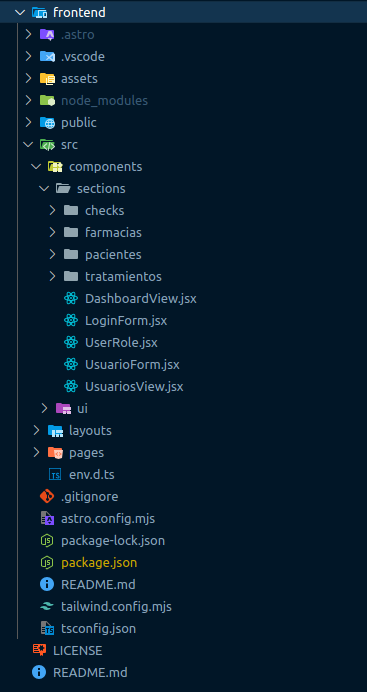
\includegraphics[width=0.5\textwidth]{imagenes/orgfront.png}
	\caption{Directorios del frontend.}
\end{figure}

\newpage
\section{Diseño de la interfaz de usuario}.
La interfaz de usuario se ha visto inspirada en el aspecto visual de un proyecto de código abierto, ScrewFast \cite{screwfast}, el cual combina el uso de Astro y Tailwind CSS para proporcionar una página web rápida y atractiva. \\

Para PharmAD predomina los colores verde, en diferentes tonalidades, y blanco. Se muestran imágenes acerca de las diferentes secciones de la plataforma.


\begin{figure}[h!]
	\centering
	
\includegraphics[width=0.9\textwidth]{imagenes/landing.png}
	\caption{Landing page.}
\end{figure}

\begin{figure}[h!]
	\centering
	
\includegraphics[width=0.9\textwidth]{imagenes/login.png}
	\caption{Pantalla de inicio de sesión.}
\end{figure}


\begin{figure}[h!]
	\centering
	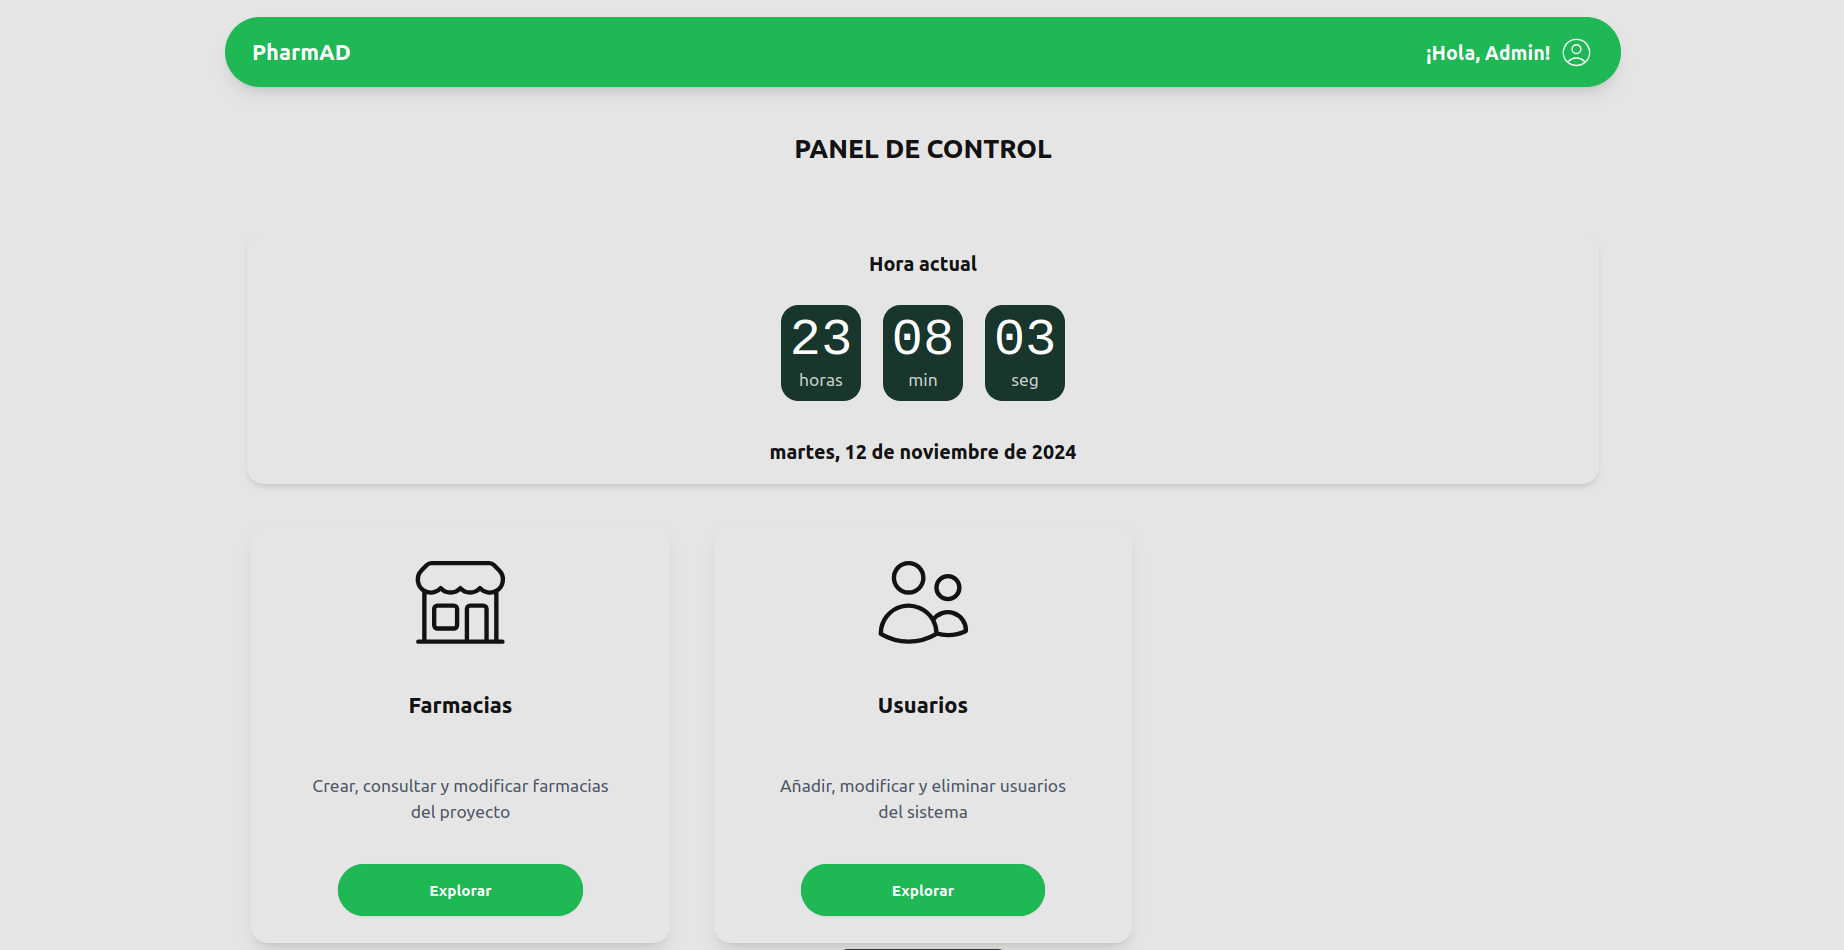
\includegraphics[width=0.9\textwidth]{imagenes/admin.png}
	\caption{Panel de control del administrador.}
\end{figure}


\begin{figure}[h!]
	\centering
	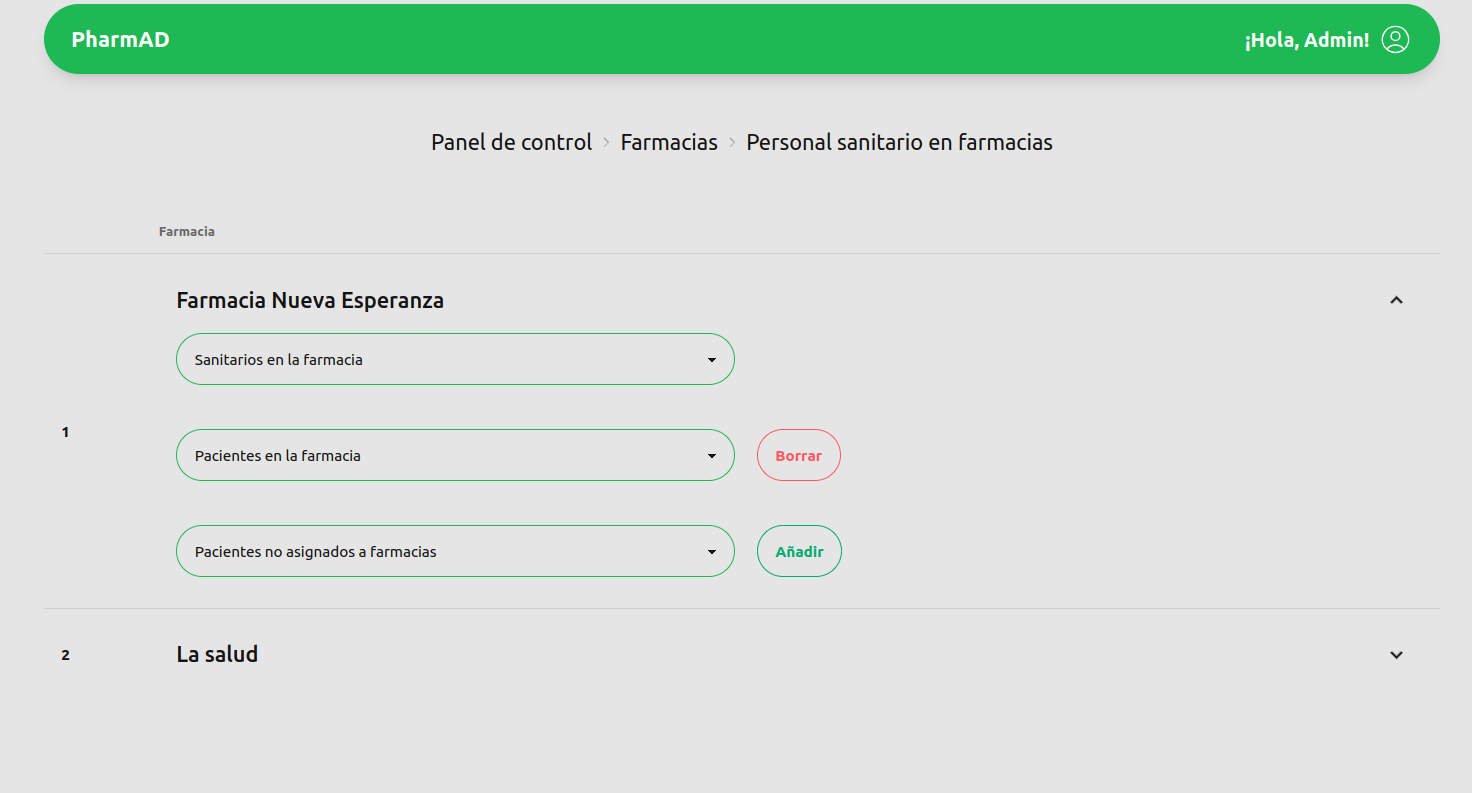
\includegraphics[width=0.9\textwidth]{imagenes/personalfarmacias.png}
	\caption{Lista de personal de farmacias para el administrador.}
\end{figure}


\begin{figure}[h!]
	\centering
	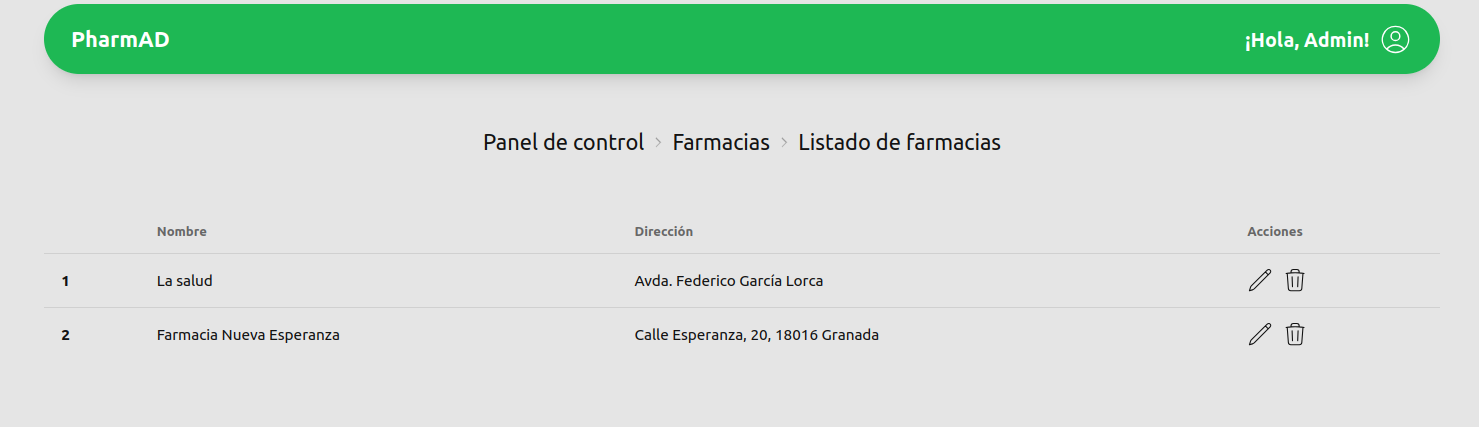
\includegraphics[width=0.9\textwidth]{imagenes/listafarmacias.png}
	\caption{Listado de farmacias para el administrador}
\end{figure}

\begin{figure}[h!]
	\centering
	
\includegraphics[width=0.9\textwidth]{imagenes/user.png}
	\caption{Panel de control del usuario.}
\end{figure}


\begin{figure}[h!]
	\centering
	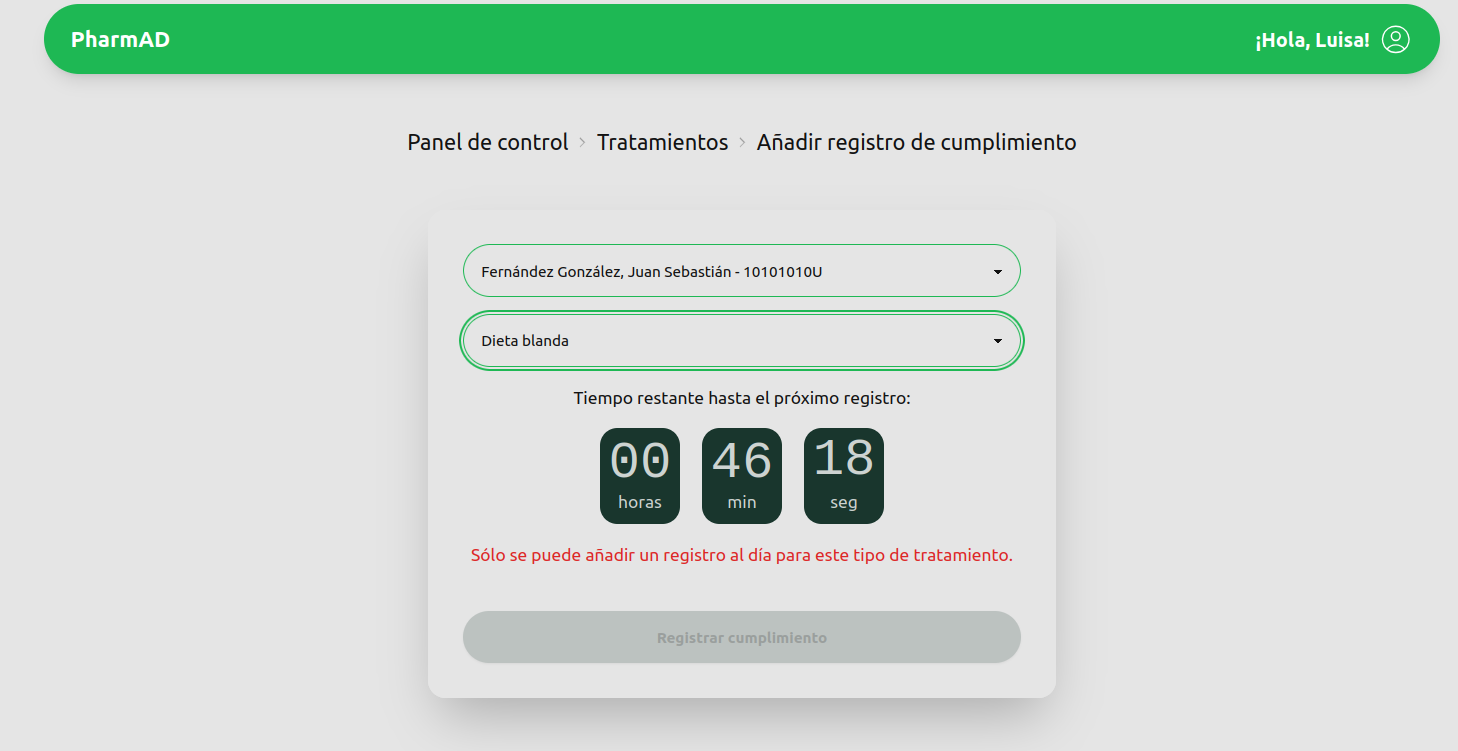
\includegraphics[width=0.9\textwidth]{imagenes/registro.png}
	\caption{Vista de registro de cumplimiento para el usuario.}
\end{figure}

\begin{figure}[h!]
	\centering
	
\includegraphics[width=0.9\textwidth]{imagenes/adherencia.png}
	\caption{Vista del informe de adherencia terapéutica para el usuario.}
\end{figure}


\begin{figure}[h!]
	\centering
	
\includegraphics[width=0.9\textwidth]{imagenes/farmaceutico.png}
	\caption{Panel de control para el farmacéutico.}
\end{figure}

\begin{figure}[h!]
	\centering
	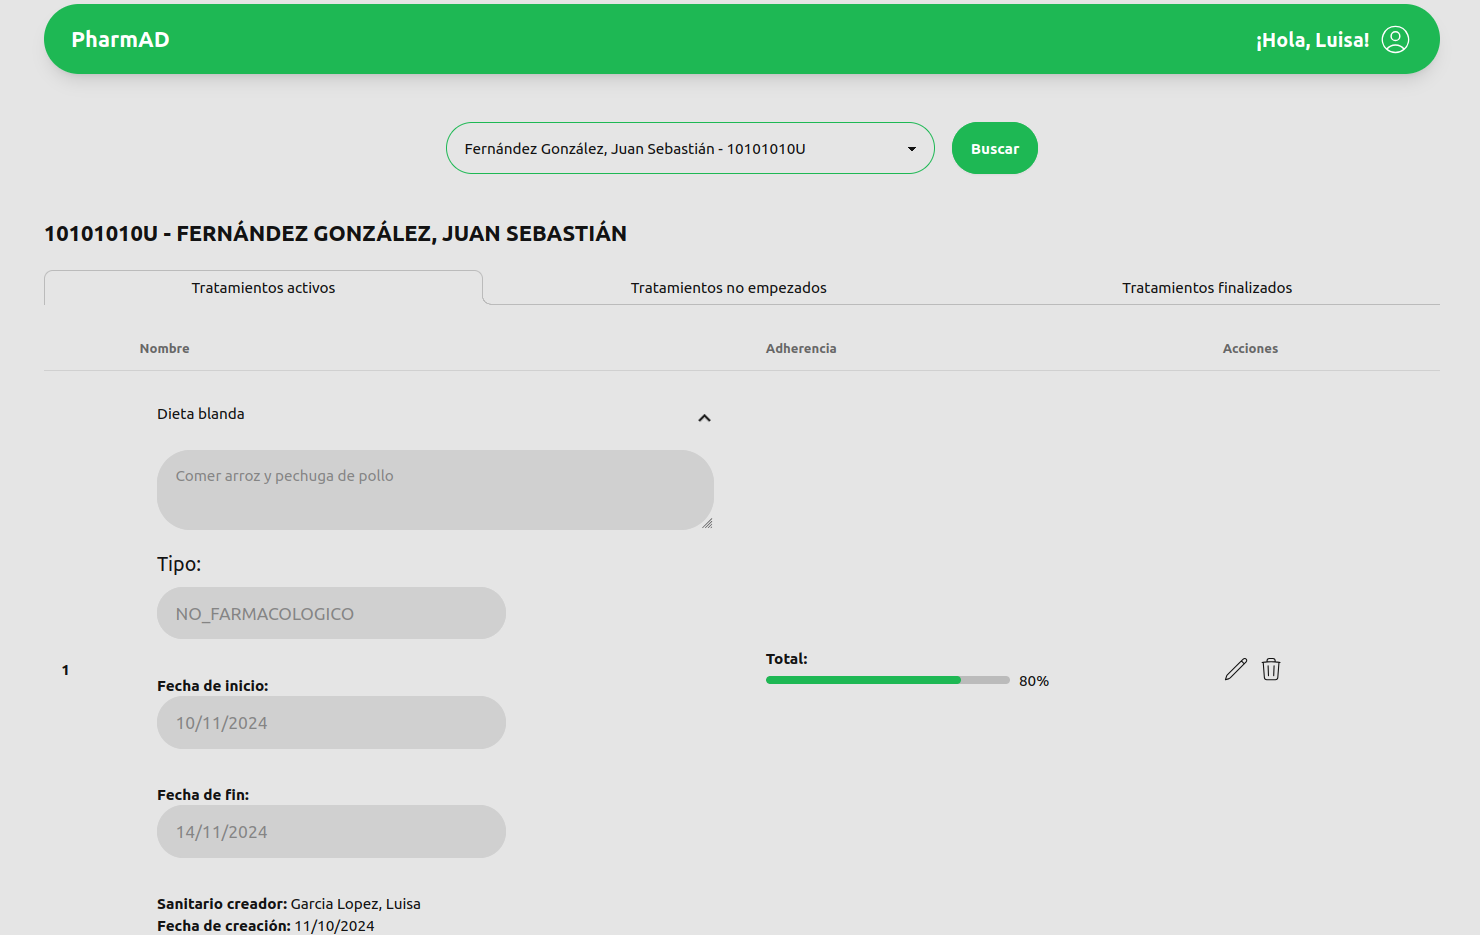
\includegraphics[width=0.9\textwidth]{imagenes/gestionarTratamientos.png}
	\caption{Vista de gestión de tratamientos para un farmacéutico.}
\end{figure}












